%!TEX root = ../../report.tex

\subsection{Tiling} % (fold)
\label{ssub:tiling}

A common solution to give realism to 3D objects is the application of textures. One problem is that this textures takes a lot of memory space. To work around this problem an easy solution is to have a small texture piece, a tile, and repeat throughout the objects. And this is called tiling. Or as defined in \cite{TilingWOLFRAM}: ``A plane-filling arrangement of plane figures or its generalisation to higher dimensions.".  This means, the result of constructing a plane from a finite set of ``tiles". 

If this technique is use naively commonly results in not very homogeneous textures, it depends much on the set of tiles that are used. If the borders of all the tiles are all the same the result is always homogeneous. But if the borders are very different the chances to have a not uniform texture rises. The Figure~\ref{fig:TIrregulartexture}, from \cite{ProcWorld} shows how a bad structured tiling system produces a not homogeneous texture.  


\begin{figure}[htbp]
	\centering
	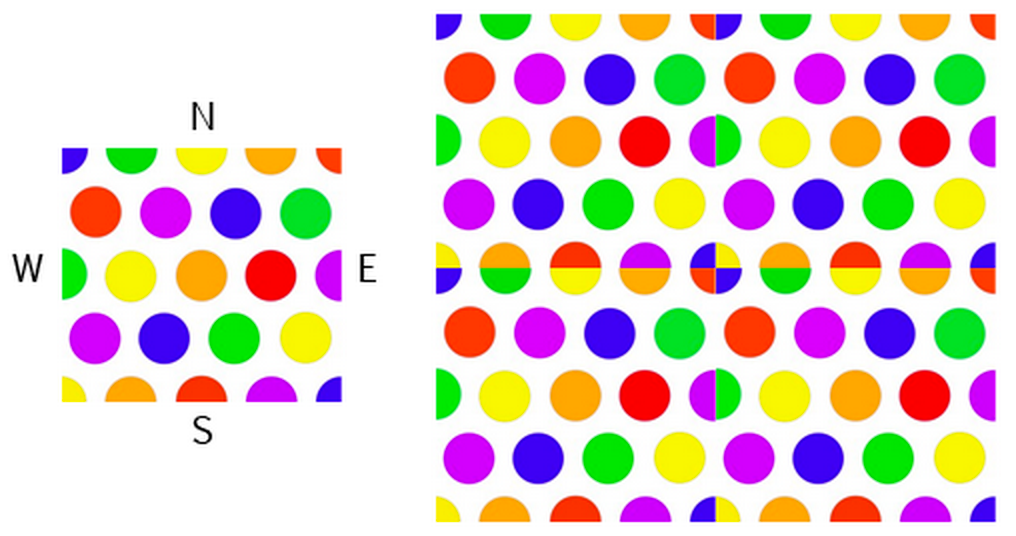
\includegraphics[width=0.95\textwidth]{img/Theory/Tiling/iregular.png}
	\caption{One tile and an irregular pattern}
	\label{fig:TIrregulartexture}
\end{figure}


To make uniform planes, the boundary of each tile must be coherent, i. e., the borders of connecting tiles have to match. Given a single tile, the so-called first corona is the set of all tiles that have a common boundary point with the tile (including the original tile itself). From that, the simple method to create a homogeneous texture is to connect each tile with one that belongs to it's first corona.

The easy, most simple solution is to make sure that all the tiles have the same borders all around. With this property it's guaranteed that any created texture will be homogeneous. But this solution doesn't provide much irregularity and the results present repeating patterns. 


\paragraph{Wang Tiles \cite{Cohen2003}.} % (fold)
\label{par:wang_tiles_}

 It is a solution named after Mr Hao Wang that predicted that tiling was not possible. It received his name, not only for him being wrong, but because the prove that this is possible uses much of the work he did trying to prove the impossibility. This process allows tiling with an arbitrary number of different vertical and horizontal borders and from that calculate the set of tiles that are needed to create a full texture without inconsistencies. 



\begin{figure}
        \centering
		\begin{subfigure}[b]{0.4\textwidth}
			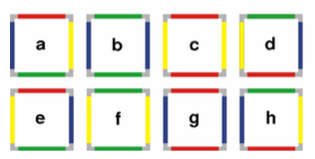
\includegraphics[width=\textwidth]{img/Theory/Tiling/tiles.png}
			\caption{a)}
			\label{fig:TTileSet}
		\end{subfigure}
        ~ ~%add desired spacing between images, e. g. ~, \quad, \qquad, \hfill etc.
          %(or a blank line to force the subfigure onto a new line)
		\begin{subfigure}[b]{0.4\textwidth}
			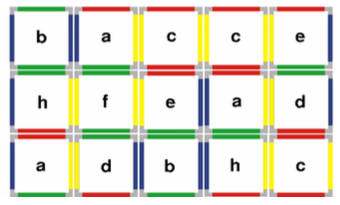
\includegraphics[width=\textwidth]{img/Theory/Tiling/plane.png}
			\caption{b)}
			\label{fig:TPlanePortion}
		\end{subfigure}
        \caption{a) Eight Wang Tiles b) Portion of a plane}
        \label{fig:WangTiles}
\end{figure}

So the process assign colors to the tiles borders and then matching colored borders are aligned forming a plane.

% paragraph wang_tiles_ (end)

As you might have noticed, the inner content of the tiles are not a problem. As we are trying to create the uniform textures by arranging this smaller pieces only the borders matter, so we can create a set of tiles with the same borders and whatever inner content we want. With this technique the result can be much more irregular and more natural looking textures.



\paragraph{Corner Tiles. \cite{LD06AWTCECC}} % (fold)
 \label{par:corner_tiles}
%One alternative to Wang tiles with the corners to be coloured.

The vanilla wang tiles have problems in the diagonals that are not taken into account. They are the confrontation between four tiles which leads to less homogeneous texture if we the borders don't match. By using the corners, the problem goes to the sides, that despite being larger, are only the confrontation between two tiles and therefore it leads to a more homogeneous texture.
 % paragraph corner_tiles (end) 


% \paragraph{Genetic tile generation} % (fold)
% \label{par:genetic_tile_generation}
% “The bottom line for me is, Wang tiles are amazing things until you try to use them seriously. They work great for stuff you can synthesise from the ground up. If you are trying to mix samples from real life, get ready for some trouble.” \cite{ProcWorld}
%\url{http://procworld.blogspot.pt/2013/01/tile-genetics.html}
% paragraph Genetic tile generation (end)




% subsubsection tiling (end)